\newpage
\section{Design Implementation}
\label{sec:design}

Our proposed design, using program graphs and channel systems, models a group of entities coordinating to complete a common goal or objective while managing dynamic events. The team's members can be diverse, due to their different set of attributes and behaviours, according to their set of roles. Moreover, due to the heterogeneity of the group, each entity can react to various situations differently, in line with its information about the environment. Also, the communication topology among the team limits their interactions and can have a large impact on the overall system. With that in mind, and following related research~\cite{evaluating} our proposed design fits as an application of an agent-based model (ABM). 

To implement our application of an ABM, we used a framework on the Java platform, \textit{Repast Symphony}~\cite{repastDoc}. The aforementioned framework is commonly used for ABM simulations~\cite{repast} and it's capacity of simulating parallelism is mandatory in our domain. Finally, the underlying object-oriented paradigm is appropriate to encapsulate each role, i.e, program graph separately, simplifying adding or removing roles throughout the execution.

We chose our motivating example (Section \ref{sec:motivation}) as the theme of our implementation. Thus, each team member and its functionalities, i.e, onboard sensors and fuel capacity, is encapsulated in a \textit{Drone} class. Also, each role is represented by a \textit{Role} class, e.g, \textit{Executor}, \textit{TaskAllocator}, and \textit{C2ApproachSelector}. Moreover, auxiliary classes were made to add modularity and functionalities, such as providing the visual communication links between members and diversify input types to start the simulation. Based on the following research~\cite{swarmGap}, we used a token-based communication protocol to exchange information among the team (class \textit{Token}), whereas the communication channels, members specification, and task allocation information are being represented by \textit{Lists}. Figure \ref{fig:ClassDiagram} shows a class diagram of the implementation.

In every round of execution, i.e, in a single time unit (tick) of the simulation, all members execute its \textit{step} method. Additionally, each member performs the \textit{step} method of its roles, which follows the program graphs described in Section 3. For instance, the task allocator (Figure \ref{fig:TA}) role class first check information inside the channel $ch_1$ to receive feedback from the executors. Next, it executes a task allocation algorithm, using the current C2 approach provided by the received Token. If the allocation process is not successful, it informs the C2 approach selector role, adding this information to the channel $ch_3$.

Similarly, the main method of the C2 approach selector role's class (\textit{step}) implements its program graph (Figure \ref{fig:C2S}). First, it checks if the task allocator role sent information along the channel $ch_3$. If a maneuver was requested, it assesses a different C2 approach using some criteria, such as defined in the following research~\cite{france2014}. In case that a change is required, it finishes execution updating maneuver variables in the Token class, asking for the team's confirmation to switch to the new C2 approach.

The full implementation and auxiliary artifacts are available in a public repository\footnote{\gitRepository}.

\begin{figure}[ht]
  \centering
  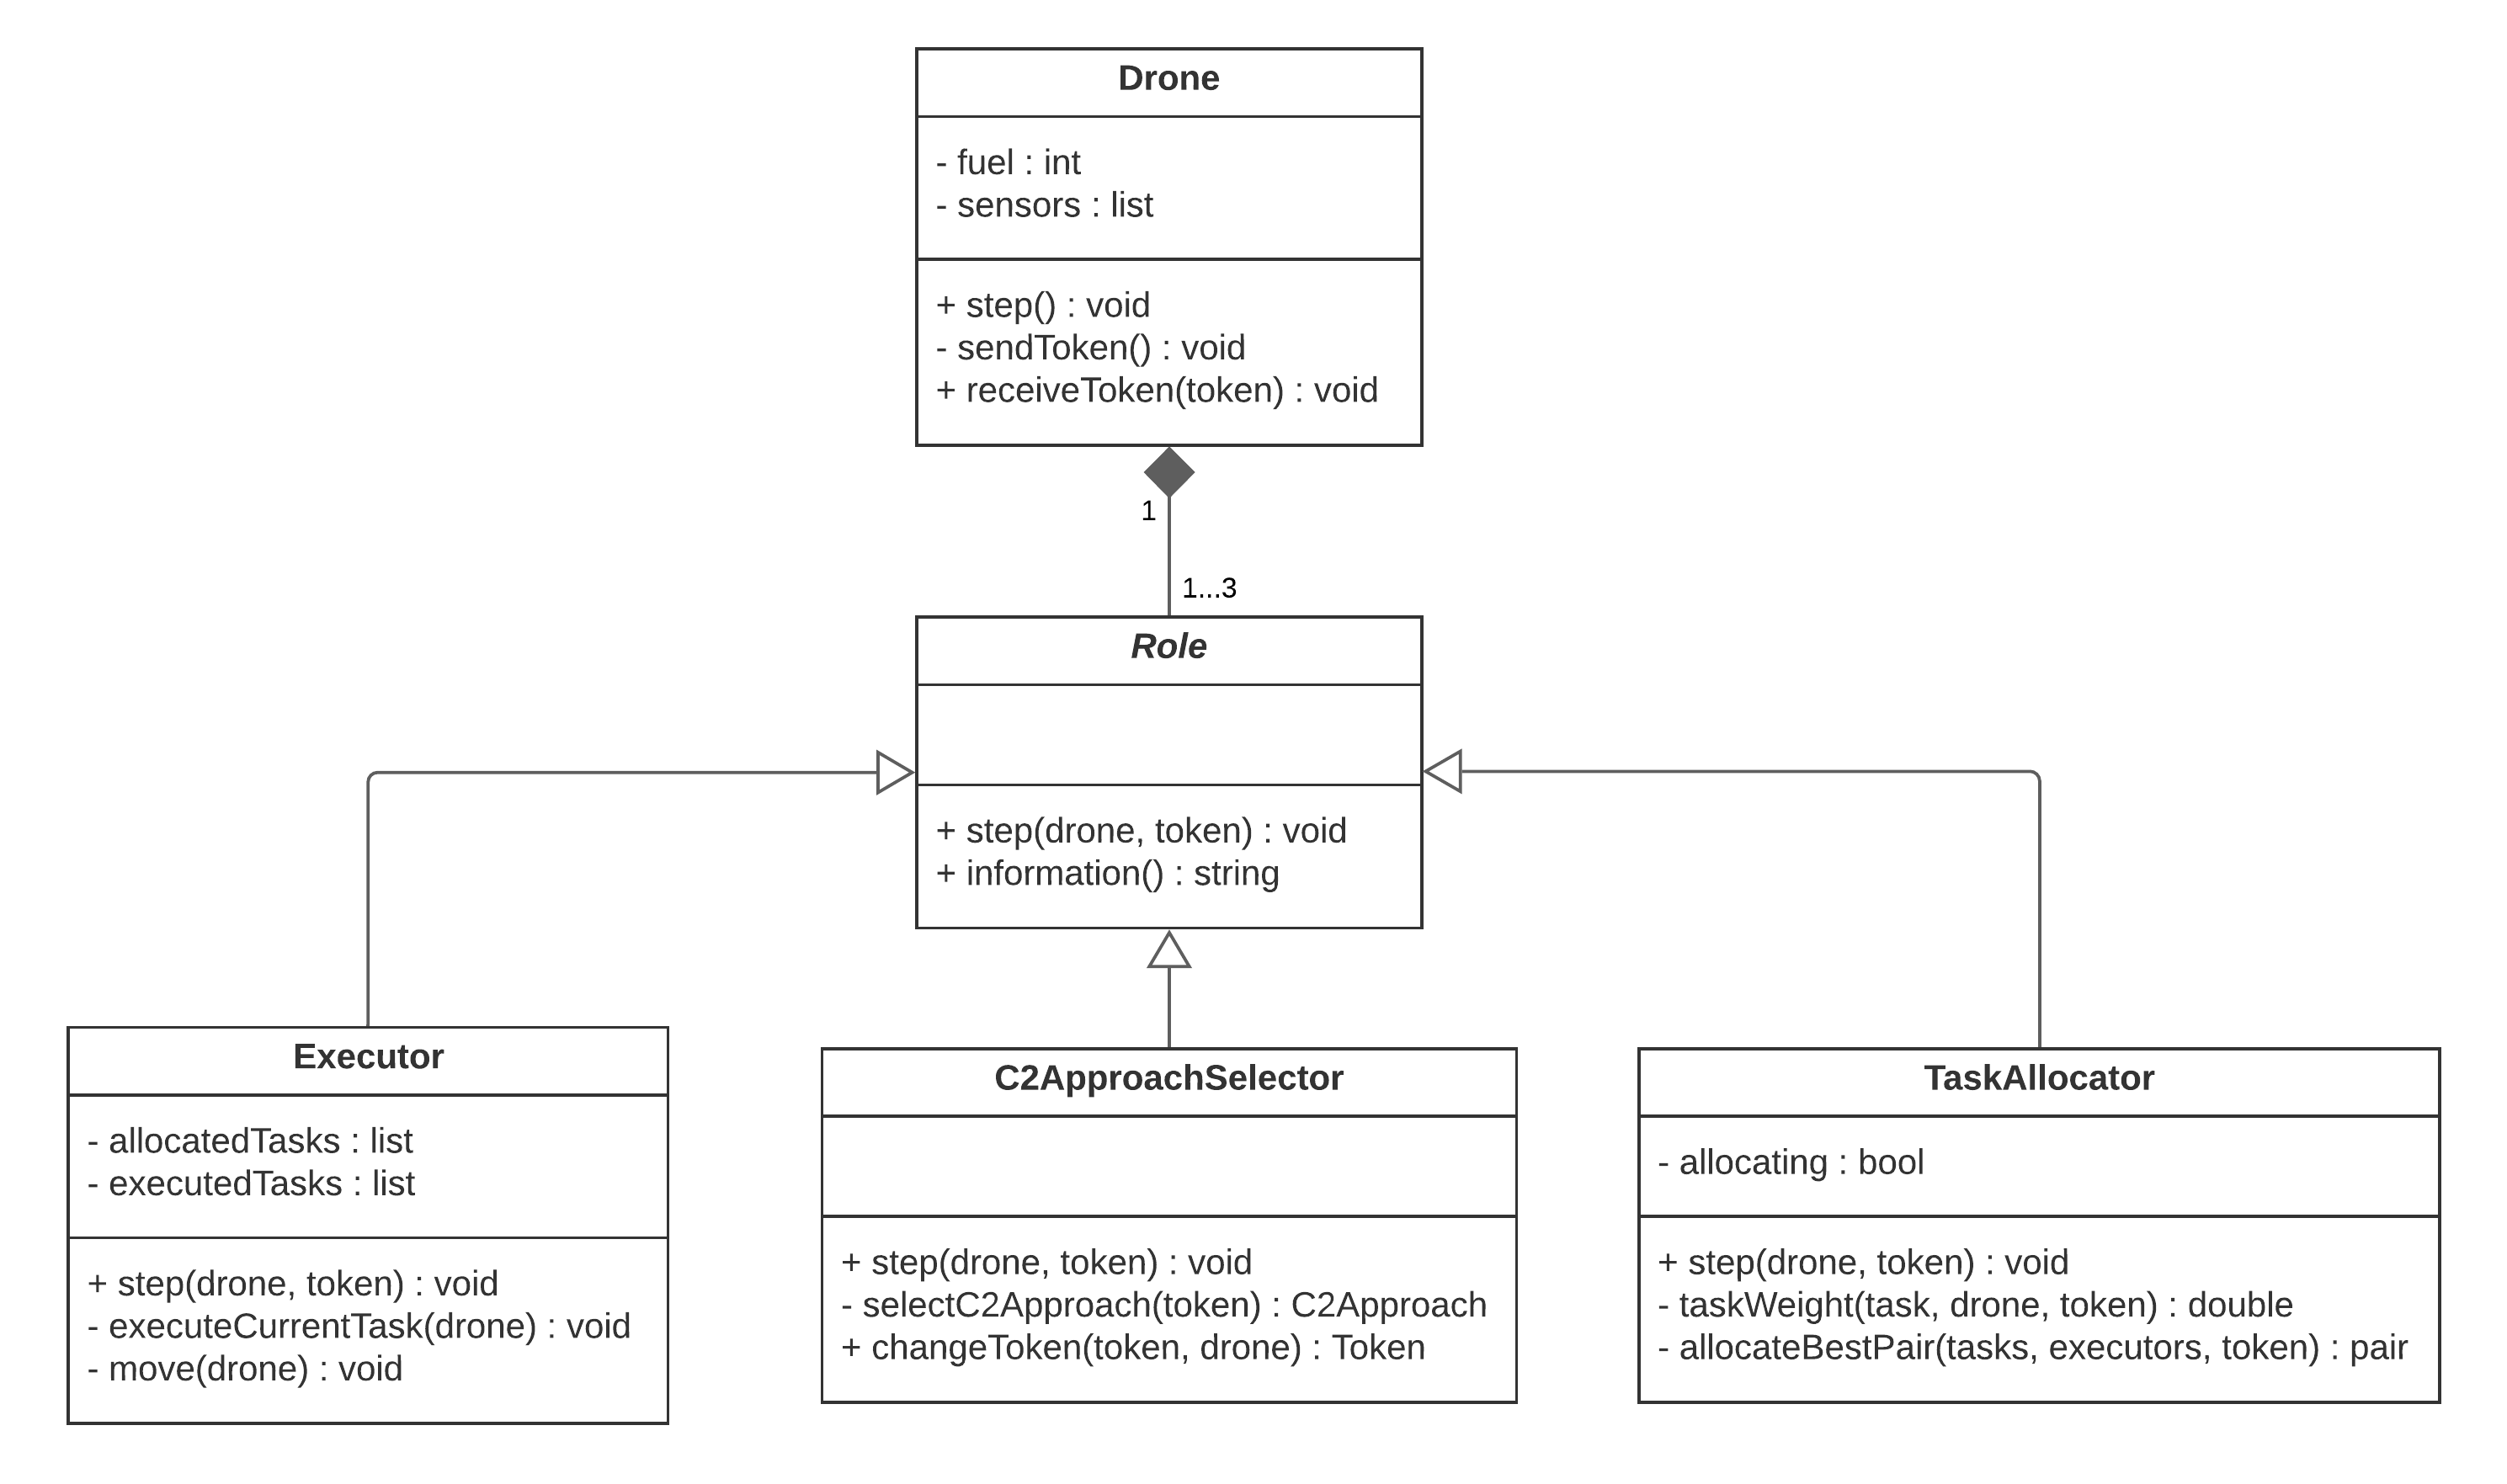
\includegraphics[width=0.9\linewidth]{figures/diagramaDeClasse.png}
  \captionof{figure}{Implementation's Class Diagram}
  \label{fig:ClassDiagram}
\end{figure}

% ROLE-BASED MODELING SECTION

% Also, because we separate a group of reusable functionalities encapsulated in different roles, our approach also applies principles from role-based modeling~\cite{roleOrientedModeling}.

% Finally, separating a group of reusable functionalities in different roles, i.e, in different program graphs, is an implementation design of role-based modeling~\cite{roleOrientedModeling, modelingAgentOrganizationsUsingRoles}.

% Roles are used to form different interfaces for agents in order to restrict the visibility of features~\cite{roleOrientedModeling}, such as internal attributes. Concerning their internal behaviour roles may capture goals and handle responsibilities~\cite{roleOrientedModeling} to execute tasks autonomously. Additionally, as demonstrated in Section \ref{subsec:PG}, roles can be dynamically attached to and retracted from an agent. This feature is especially important if a role shall migrate from one agent to another~\cite{roleOrientedModeling} in run time. For instance, when a maneuver occurs some agents may undergo a complete transformation in its roles, depending on the role of the C2 approach selector to decide which set of roles is more appropriate for each agent.

% A role class can be described in terms of its breath and dept~\cite{modelingAgentOrganizationsUsingRoles}. Breadth, or horizontal specialization, addresses the number and complexity of actions supported by a given role~\cite{modelingAgentOrganizationsUsingRoles}. Depth, or vertical specialization, relates to the degree of control an agent can have over its actions and the actions of other agents~\cite{modelingAgentOrganizationsUsingRoles}. Recalling Section \ref{sec:introduction}, horizontal specialization is more related to C2 Approach Agility, due to its nature of providing agility within the same C2 approach, adding resilience and flexibility in the current structure of execution. Similarly, vertical specialization relates to C2 Maneuver Agility. Dept relates to the task allocator and C2 approach selector roles, due to their level of influence over the remaining members while performing a maneuver or even which tasks they will execute.
